\documentclass{standalone}
\usepackage{tikz}
\usepackage{ctex,siunitx,ninecolors}
\setCJKmainfont{Noto Serif CJK SC}
\usepackage{tkz-euclide}
\usepackage{amsmath}
\usepackage{wasysym}
\usetikzlibrary{patterns, calc}
\usetikzlibrary{decorations.pathmorphing, decorations.pathreplacing, decorations.shapes,3d}
\newcommand{\posthead}[2][gray]{
  \begin{tikzpicture}[#2]
    \fill[left color=#1,right color= #1,middle color=#1!20](0,0)ellipse(0.05 and 0.02);
    \fill[left color=#1,right color= #1,middle color=#1!20](0.05,0)rectangle(-0.05,0.07);
    \fill[left color=#1,right color= #1,middle color=#1!20](-0.06,0.07)arc(-180:0:0.06 and 0.02)--(0.06,0.15)--(0.05,0.16)--(-0.05,0.16)--(-0.06,0.15)--cycle;
    \fill[#1!50!gray](0,0.16)ellipse(0.05 and 0.02);
    \foreach \x in {75,45,15,-15,-45,-75}
    {
      \draw[very thin,#1!50!gray]({0.05*sin(\x)},{0.16-0.02*cos(\x)})--({0.06*sin(\x)},{0.15-0.02*cos(\x)})--++(0,-0.08);
    }
  \end{tikzpicture}
}
\begin{document}
\small
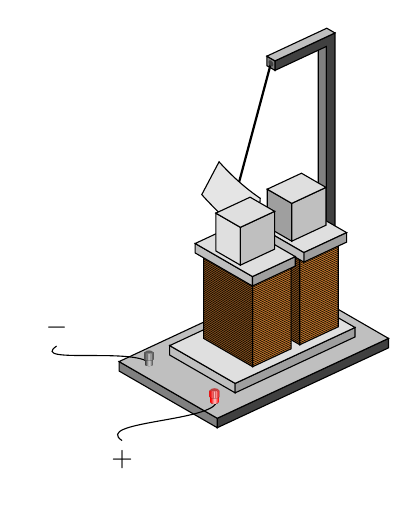
\begin{tikzpicture}[>=latex,scale=1.2]
  \begin{scope}[z={(25:10mm)},x={(150:10mm)}]
    \begin{scope}[canvas is yz plane at x=-0.6]
      \draw[fill=darkgray](0,-1)rectangle(-0.1,1);
    \end{scope}
    \begin{scope}[canvas is xy plane at z=-1]
      \draw[fill=gray](0.6,-0.1)rectangle(-0.6,0);
    \end{scope}
    \begin{scope}[canvas is zx plane at y=0]
      \draw[fill=lightgray](-1,-0.6)rectangle(1,0.6);
    \end{scope}
    \begin{scope}[canvas is xy plane at z=0.8]
      \draw[fill=gray](0.05,2.9)rectangle(-0.05,0);
    \end{scope}
    \begin{scope}[canvas is yz plane at x=-0.05]
      \draw[fill=darkgray](0,0.9)--(3.0,0.9)--(3.0,0.2)--(2.9,0.2)--(2.9,0.8)--(0,0.8)--cycle;
    \end{scope}
    \begin{scope}[canvas is xy plane at z=-0.6]
      \draw[fill=gray!50](0.4,0.1)rectangle(-0.4,0);
    \end{scope}
    \begin{scope}[canvas is yz plane at x=-0.4]
      \draw[fill=darkgray!50](0,-0.6)rectangle(0.1,0.8);
    \end{scope}
    \begin{scope}[canvas is zx plane at y=0.1]
      \draw[fill=lightgray!50](-0.6,-0.4)rectangle(0.8,0.4);
    \end{scope}

    \begin{scope}[canvas is xy plane at z=0.25]
      \draw[fill=brown4](0.3,0.1)rectangle(-0.3,1);
      \foreach \x in {0.12,0.14,...,0.99}{\draw[very thin](-0.3,\x)--(0.3,\x);}
      \draw[fill=gray!50](0.35,1.1)rectangle(-0.35,1);
    \end{scope}
    \begin{scope}[canvas is yz plane at x=-0.3]
      \draw[fill=brown6](1.0,0.25)rectangle(0.1,0.7);
      \foreach \x in {0.12,0.14,...,0.99}{\draw[very thin](\x,0.25)--(\x,0.7);}
    \end{scope}
    \begin{scope}[canvas is zx plane at y=1.1]
      \draw[fill=lightgray!50](0.25,-0.35)rectangle(0.75,0.35);
    \end{scope}
    \begin{scope}[canvas is yz plane at x=-0.35]
      \draw[fill=darkgray!50](1.0,0.25)rectangle(1.1,0.75);
    \end{scope}
    \begin{scope}[canvas is xy plane at z=0.25]
      \draw[fill=gray!50](0.35,1.1)rectangle(-0.35,1);
    \end{scope}
    \begin{scope}[canvas is xy plane at z=0.3]
      \draw[fill=darkgray!50](0.15,1.1)rectangle(-0.15,1.5);
    \end{scope}
    \begin{scope}[canvas is yz plane at x=-0.15]
      \draw[fill=gray!50](1.1,0.3)rectangle(1.5,0.7);
    \end{scope}
    \begin{scope}[canvas is zx plane at y=1.5]
      \draw[fill=lightgray!50](0.3,-0.15)rectangle(0.7,0.15);
    \end{scope}

    \begin{scope}[canvas is xy plane at z=0.2]
      \draw[fill=gray](-0.05,2.9)rectangle(0.05,3);
      \draw[thick](0,2.95)--++(-75:1.5);
      \fill[darkgray](0,2.95)circle(0.03);
      \draw[fill=lightgray!40]([shift=(-65:2.0)]0,2.95)arc(-65:-85:2.0)--++(-85:-0.5)arc(-85:-65:1.5)--cycle;
    \end{scope}

    \begin{scope}[canvas is yz plane at x=-0.3]
      \draw[fill=brown6](1.0,-0.3)rectangle(0.1,0.15);
      \foreach \x in {0.12,0.14,...,0.99}{\draw[very thin](\x,-0.3)--(\x,0.15);}
    \end{scope}
    \begin{scope}[canvas is xy plane at z=-0.3]
      \draw[fill=brown4](0.3,0.1)rectangle(-0.3,1);
      \foreach \x in {0.12,0.14,...,0.99}{\draw[very thin](-0.3,\x)--(0.3,\x);}
    \end{scope}
    \begin{scope}[canvas is xy plane at z=-0.35]
      \draw[fill=gray!50](0.35,1.1)rectangle(-0.35,1);
    \end{scope}
    \begin{scope}[canvas is yz plane at x=-0.35]
      \draw[fill=darkgray!50](1.0,-0.35)rectangle(1.1,0.15);
    \end{scope}
    \begin{scope}[canvas is zx plane at y=1.1]
      \draw[fill=lightgray!50](-0.35,-0.35)rectangle(0.15,0.35);
    \end{scope}

    \begin{scope}[canvas is xy plane at z=-0.3]
      \draw[fill=lightgray!50](0.15,1.1)rectangle(-0.15,1.5);
    \end{scope}
    \begin{scope}[canvas is yz plane at x=-0.15]
      \draw[fill=gray!50](1.1,-0.3)rectangle(1.5,0.1);
    \end{scope}
    \begin{scope}[canvas is zx plane at y=1.5]
      \draw[fill=lightgray!50](-0.3,-0.15)rectangle(0.1,0.15);
    \end{scope}

    \begin{scope}[canvas is zx plane at y=3]
      \draw[fill=lightgray](0.2,-0.05)rectangle(0.9,0.05);
    \end{scope}
    \coordinate (A) at (0.5,0,-0.8);
    \coordinate (B) at (-0.3,0,-0.8);
  \end{scope}
  \draw([shift=(-45:0.1)]A)..controls++(-0.1,0.2)and++(-0.3,-0.2)..++(-1,0.2)node[above]{$-$};
  \draw([shift=(-45:0.1)]B)..controls++(-0.1,-0.2)and++(-0.3,0.2)..++(-1,-0.4)node[below]{$+$};
  \node at (A)[inner sep=0pt] {\posthead[darkgray]{}};
  \node at (B)[inner sep=0pt] {\posthead[red]{}};
\end{tikzpicture}
\end{document}